%%%%%%%%%%%%%%%%%%%%%%%%%%%%%%%%%%%%%%%%%%%%%%%%%%%%%%%%%%%%%%%%%%%%%%%%%%%%%%%%%%%%%%%%%%%%%%%%%%%%
% NONLINEAR THEORY 
%%%%%%%%%%%%%%%%%%%%%%%%%%%%%%%%%%%%%%%%%%%%%%%%%%%%%%%%%%%%%%%%%%%%%%%%%%%%%%%%%%%%%%%%%%%%%%%%%%%%
\chapter{Nonlinear simulations}

\section{Introduction}
In the previous chapter, we investigated the linear stability of the Lamb-Chaplygin dipole and we showed that the short-wave instability can have growth rates that are comparable to those of the zigzag instability. An important question is if both of these instabilities exist, which will dominate in the transition to turbulence? In the atmosphere and ocean, a wide range of length scales are excited, so it is expected that both the zigzag instability and the short-wave instability will be excited in nature. Understanding the evolution of these two instabilities and what role they play in the transition to turbulence is important to correctly understand the mechanisms at play in the transition to stratified turbulence. Unfortunately, as alluded to in Chapter 2, linear stability analysis can only take us so far. 

In this chapter we evolve the full nonlinear Boussinesq equations to determine how the short-wave instability evolves and what role it plays in the transition to turbulence. The importance of the zigzag instability in the breakdown and transition to turbulence has been well studied \cite{augier2012,waitesmol2008,augierbillant2011,delonclebc2008} and none of these studies have mentioned short-wavelength instabilities. In this chapter we investigate the role of the short-wave instability in the transition to turbulence. Through nonlinear simulations, we will demonstrate that the saturation level of the short-wave instability is relatively small and depends upon the aspect ratio $\delta=L_{v}/L_{h}$. Thus, for many geophysical flows, where $\delta\ll 1$, the short-wave instability may not affect the overall breakdown and transition to turbulence. 

\section{Set-up} 
To investigate the nonlinear evolution, we use a code developed by Waite \cite{waite2011}; the parallel version of the code was developed by Bartello \cite{bartello1995}. The code implements the spectral method technique discussed in Chapter 3 to solve the nonlinear Boussinesq equations. Unlike in linear stability analysis, nonlinear analysis of the Boussinesq equations is much more complicated as particular attention must be taken to ensure proper resolution of the small scales. The breakdown of the zigzag instability exhibits small scale turbulence \cite{augier2012} which suggests that we might observe a similar result for the short-wave instability. Thus we need to choose grid sizes that resolve the smallest scales of such turbulence, known as the Kolmogorov scale. 

The Kolmogorov scale is given by \cite{lesieur}
\begin{align}
\eta = \left(\frac{\nu^{3}}{\epsilon}\right)^{3},
\end{align}
where $\epsilon$ is the kinetic energy dissipation rate, which is commonly approximated as \cite{lindborg2006}
\begin{align}
\epsilon \sim \frac{U^{3}}{R} ,
\end{align}
where $U,R$ are the characteristic velocity and length respectively. Rewriting the Kolmogorov scale $\eta$ in terms of the Reynolds number by multiplying by the characteristic length $R$ we obtain
\begin{align}
\frac{\eta}{R} = \frac{1}{\Re^{3/4}}.
\end{align}
We want to choose the number of grid points to be such that the horizontal and vertical grid spacings satisfy $\Delta x \approx \Delta z \approx \eta/R$, where the factor of $R$ takes into account the $\Delta x, \Delta z$ are the grid spacings of the dimensionless equations (give eqn numbers).

To focus specifically on the short-wave instability, we choose the vertical scale to be that of the short-wave instability. To illustrate, consider $Re=2000, F_{h}=0.2$ where the short-wave instability peaks at $k_{z}=20$. Here we set the vertical domain size to be one vertical wavelength of the short-wave instability, i.e.
\begin{align}
L_{v} = \frac{2\pi}{k_{z}} = \frac{2\pi}{20}.
\end{align}
From our linear results, we again take $L=9$. Due to the set-up of the code, the number of grid points in every direction has to be a power of small primes; we choose powers of $2$. Thus let us a priori consider the number of horizontal grid points to be $n_{x}=1024$. We have that the horizontal resolution is
\begin{align}
\Delta x = \frac{L}{n_{x}} = \frac{9}{1024}\approx 0.00878,\qquad \frac{\eta}{R}\sim \frac{1}{Re^{3/4}}=0.003343,
\end{align}
and we approximately have that $\Delta x \sim \eta/R$. In nonlinear simulations of the zigzag instability, Augier et al.\cite{augierbillant2011} used $n_{x}=512$ with $Re=2500$ and $L=10$; our resolution is slightly higher. If choose $n_{z}=32$ grid points in the vertical, we find that $\Delta z \approx 0.00982$ which is very similar to $\Delta x$. For our timestep we choose $\Delta = 5.0\times 10^{-4}$. Each run was initialised with a random density sinusoidal perturbation with $\epsilon=0.01$. 

\section{Results}
As mentioned in the introduction, previous investigations into the transition of turbulence have focused only on the zigzag instability. In all these simulations, it is clear that the dominant instability is the zigzag instability. For example, in Waite and Smolarkiewicz \cite{waitesmol2008}, the growth rates of the zigzag instability agree with the linear theory. It is possible that these simulations were not resolving the small scales, although this does not seem likely based on the parameters given. This is because the length scale of the short-wave instability is about an order of magnitude or so smaller than that of the zigzag instability. Since these simulations were intended to study the transition to turbulence, they would be resolving, or close to resolving, the Kolmogorov scale, which is much smaller than the short-wave instability. Hence it is unlikely a resolution issue. Instead, it could be the case that the short-wave instability is present but saturates out and does not contribute significantly to the transition to turbulence. We explore this option here. 

Consider the following scaling argument and results due to Ngan et al.\cite{ngan2005}. They were interested in three-dimensionalisation of a two-dimensional flow in small aspect ratio domains, which they referred to as quasi-two-dimensional turbulence. They considered this as they were interested in geophysical flows which exhibit small aspect ratios, $\delta=0.01-0.1$ \cite{ngan2005}. As we have seen, stratified turbulence tends to have a small aspect ratio and, as discussed in Chapter 2, exhibits characteristics of geophysical flow. However, it is important to note that Ngan et al.\cite{ngan2005} did not consider stratification and they were only focusing on the unstratified case of turbulence with small aspect ratios. 

To investigate this three-dimensionalisation, in their numerical experiments they took fully developed 2D turbulence and subjected it to a 3D perturbation. They then measured the saturation level of this 3D perturbation. The saturation level is defined to be
\begin{align}
\text{saturation} = \frac{u}{U}\bigg|_{t=sat}, \label{ngan_scale}
\end{align}
where the ratio between the 3D rms velocity $u$ and the 2D rms velocity $U$ are evaluated at the saturation time. The saturation time is the time at which the time series of the 3D rms velocity levels off or saturates. They found, numerically, that this saturation level depended linearly on the aspect ratio $\delta$, up to a certain aspect ratio, $\delta=0.5$. Beyond $\delta=0.5$ the numerical simulations could no longer be considered quasi-two dimensional. 

To explain this result, Ngan et al.\ considered a simple scaling argument \cite{ngan2004,ngan2005}. Initially the time scales of the 2D base flow is long compared to that of the 3D perturbation flow. However once the 3D perturbation settles down and saturates, its timescale becomes similar to that of the 2D flow.  Consider the following timescales for these flows \cite{ngan2005} as
\begin{align}
T_{2D} = \frac{U}{L},\qquad T_{3D} =\frac{u}{H},
\end{align}
where $U$ is the characteristic velocity of the 2D flow at saturation and $u$ is the characteristic velocity of the 3D flow at saturation. At saturation $T_{2D}\sim T_{3D}$ and thus we have that 
\begin{align}
\frac{U}{L}\sim\frac{u}{H} \Rightarrow \frac{u}{U} \sim \frac{H}{L} = \delta,
\end{align}
which is the result they confirmed numerically. 

Motivated by this result, we consider the saturation levels of the short-wave instability for $Re=2000,5000$ and $F_{h}=0.2$. These two cases were chosen as they both had short-wave instability growth rates similar to that of the zigzag peak. Higher $Re$ could not be explored due to resolution issues, as alluded to in the previous section. 

There are different strategies available for determining the perturbation energy in these simulations. One approach is to compute the 2D and 3D rms velocities using the vertical wavenumber $k_{z}$\footnote{This is the vertical wavenumber of the nonlinear simulation, not that of the short-wave instability.} kinetic energy spectrum. The two-dimensional kinetic energy is in $k_{z}=0$; the three-dimensional kinetic energy is the contribution from all non-zero $k_{z}$. 

However, a simpler approach is to use the potential and kinetic energy, since the potential energy is entirely due to the pertrubation, while (at early times at least) the kinetic energy is mainly due to the dipole.

Both methods were used to compute the saturation level and it was found that the results using the kinetic and potential energy collapsed better than those of the 2D and 3D kinetic energy. [Fig.~\ref{sat_energy} demonstrates the evolution of these quantities for $Re=5000, F_{h}=0.2, k_{z}=40$. As can be observed, the total kinetic and 2D kinetic energies are nearly indistinguishable. The 3D kinetic and potential energies have similar amplitude and trend, but the saturation level seems clearer and better defined in the potential energy. For this reason, we choose to use the potential energy to identify the saturation level. Despite the differences, both curves have the same saturation time, roughly $T=20$. For the parameters investigated, the saturation time was approximately $T=20$. 
\begin{figure}
\begin{center}
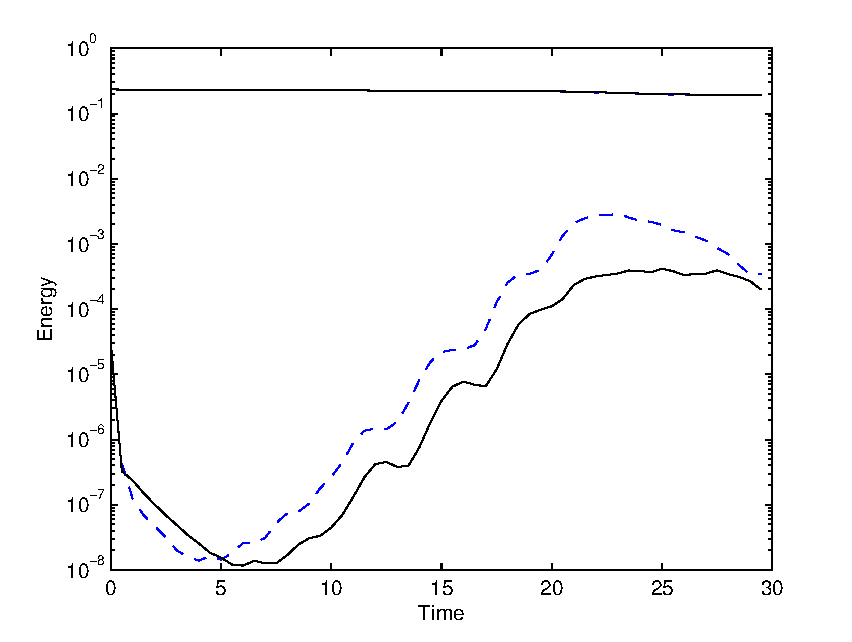
\includegraphics[width=\textwidth]{sat_eg_re5000_fh02}
\caption{Time series demonstrating the two ways of computing the energy for $Re=5000, F_{h}=0.2$, and $k_{z}=40$. The blue curves correspond to the kinetic energy seperated into 2D (solid) and 3D (dashed); the black curves are the total kinetic energy (solid) and potential energy (dashed). All energies are domain averages.}
\label{sat_energy}
\end{center}
\end{figure}
Nevertheless, it is still interesting to consider the evolution of the contributions to the kinetic energy from different vertical wavenumbers. Fig.~\ref{other_kz} demonstrates this for the paramters given above. Here we can explicitly see which wavenumbers are contributing to the total 3D kinetic energy. For almost the entire simulation, the primary vertical mode $(k_{z}=20)$ domainted. However at around the saturation time $T=20$, $k_{z}=2\times 20$ appears to make a small, but noticeable contribution to the total 3D kinetic energy. This lasts for about $5$ time units before diffusion begins to rapdily diffuse out the smaller scales, which is especially evident in the highest wavenumbers. 
\begin{figure}
\begin{center}
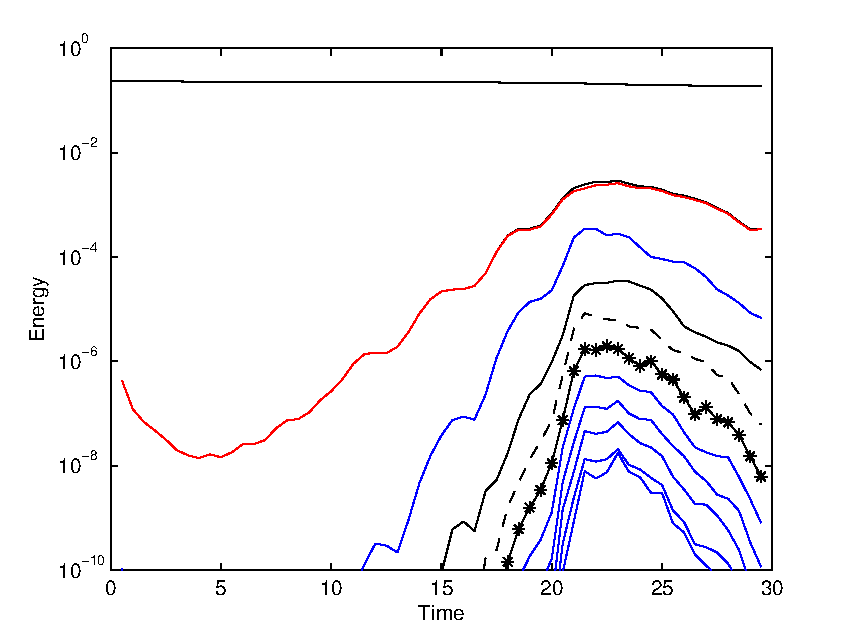
\includegraphics[width=\textwidth]{other_kz}
\caption{Time series for the contribution from different vertical wavenumbers for $Re=5000, F_{h}=0.2$, and $k_{z}=40$. The top black curve corresponds to $k_{z}=0$, i.e. the 2D kinetic energy. The remaining curves correspond to $k_{z} = 40n$ where $n=1$ (red), $2$ (blue), $3$ (black), etc. The black curve that is obscured by the red line is the total 3D kinetic energy.}
\label{other_kz}
\end{center}
\end{figure}

To determine the saturation level as a function of $\delta$, we performed a number of simulations of the short-wave instability perturbed at a range of $k_{z}$ values around the short-wave peak for $Re=2000,5000, F_{h}=0.2$. Fig.~\ref{re2000sat} is the case of $Re=2000$. As found by Ngan et al.\cite{ngan2005}, the saturation level increases for increasing delta. Using a least-squares fit we find that the best fit curve is $\delta^{3.02}$ and have plotted a reference curve of slope $3$. Fig.~\ref{re5000sat} is the case of $Re=5000$. Again, the trend of saturation level with increasing aspect ratio is observed here. Using a least-squares fit we find that the best fit curve is $\delta^{3.16}$ and a reference curve of slope $3$ is plotted. At this higher Reynolds number, it was observed that although the saturation was clear, the actual time to choose to evaluate the saturation ratio was not well defined. In Fig.~\ref{sat_energy} although the saturation level here is fairly flat, there is still a bit of variation in the saturation level. In some cases this variation was more pronounced so defining where to evaluate the saturation ratio was not well defined. For consistency, the first maximum after $T=20$ times unit was chosen. 

\begin{figure}
\begin{center}
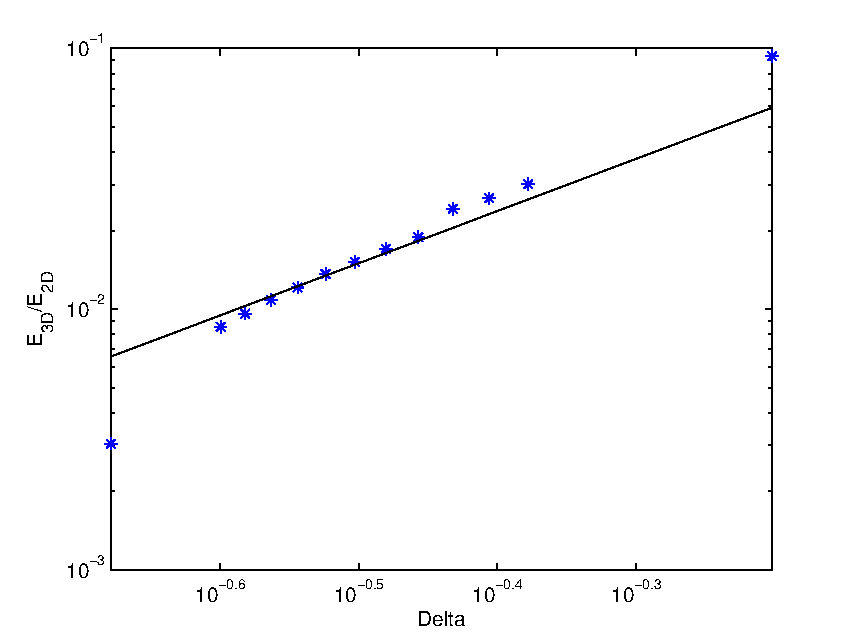
\includegraphics[width=\textwidth]{re2000_fh02_saturations} 
\caption{Saturation levels for a range of aspect ratios $\delta$ for $Re=2000$ and $F_{h}=0.2$. The curve has slope $3$.}
\label{re2000sat}
\end{center}
\end{figure}
\begin{figure}
\begin{center}
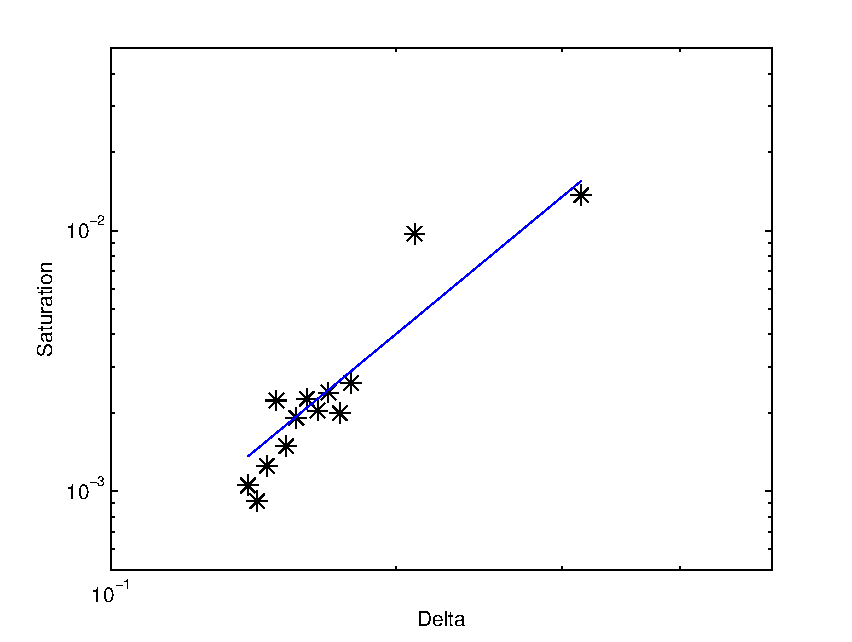
\includegraphics[width=\textwidth]{re5000_fh02_saturation_levels} 
\caption{Saturation levels for a range of aspect ratios $\delta$ for $Re=5000$ and $F_{h}=0.2$. The curve has slope $3$. }
\label{re5000sat}
\end{center}
\end{figure} 
From these two curves it suggests that the saturation level of the short-wave instability is given by
\begin{align}
\frac{E_{2D}}{E_{3D}}\bigg|_{t=sat} \sim \delta^{3},
\end{align}
which suggests that as the aspect ratio decreases, the saturation level decreases. From the linear theory, the wavenumber of maximum short-wave instability was found to scale as $k_{z}\sim F_{h}^{-1/5}Re^{2/5}$ or $k_{z}'\sim F_{h}^{-1/5}Re^{2/5}/R$ in dimensional units. Then the aspect ratio scales as $\delta = 2\pi(k_{z}R) \sim F_{h}^{1/5}Re^{-2/5}$ and hence the saturation level is 
\begin{align}
\frac{E_{2D}}{E_{3D}}\bigg|_{t=sat} \sim (2\pi)^{3}F_{h}^{3/5}Re^{-6/5}.
\end{align}
Plugging in $Re=5000$ and $F_{h}=0.2$ yields a ratio on the order of $10^{-3}$ which agrees with Fig.~\ref{sat_energy}. For $F_{h}\ll 1$ and $Re\gg 1$ this ratio is $\ll 1$. Thus given that the short-wave instability seems to saturate at a relatively low level, we should not expect the short-wave instability to play a significant role in the evolution of the Lamb-Chaplygin dipole's transition to turbulence. 

This scaling for the saturation level differs from that of Ngan et al.\cite{ngan2005}. If we square Eq. (\ref{ngan_scale}) we obtain 
\begin{align}
\frac{u^{2}}{U^{2}} =\frac{KE_{3D}}{KE_{2D}}\sim \delta^{2},
\end{align}
which suggests that the saturation level will scale quadratically instead of cubically. %However, despite the difference in exponents, we do observe similar trends to Ngan et al.\cite{ngan2005} in 

%It is clear that their simple dimensional argument breaks down when stratification occurs, but this is not too surprising since the origins of their argument \cite{ngan2004} is based on a ``pressureless" argument where 
%\begin{align}
%\frac{|\nabla_{h}p|}{|\bm{u}\nabla\bm{U}|}= \mathcal{O}(\delta^{2}).
%\end{align}
%Using our scaling from Chapter 4, we would find, with $\rho_{0}=1$ following \cite{ngan2004}
%\begin{align}
%\frac{|\nabla_{h}p|}{|\bm{u}\nabla\bm{U}|}= \mathcal{O}(\delta^{-1}),
%\end{align}
%which is very different. Thus, we cannot use their scaling argument here. However, the similarities in results does suggest that such a dimensional argument might be possible.

Fig.~\ref{full_structure} is the vertical vorticity at three times, $T=15,20,25$. Just before saturation $(T=20)$ the structure of the dipole does not exhibit any small-scale features. However at $T=20$, the saturation time, the dipole exhibits many small-scale features. By $T=25$ they appear to have been diffused out and the structure of the dipole has returned to one similar to before saturation, albeit with the two cores of the dipole more homogeneous in vorticity. The structure suggests that the saturation time is important as the dipole is undergoing some sort of transition, but as we saw, this transition is short lived as $5$ time units later, small-scale behaviour has diffused out and there is no suggestion that the system will transition to turbulence. Indeed, this result reaffirms that the gridspacing is sufficient enough to resolve the nonlinear evolution. 

\begin{figure}
\begin{center}
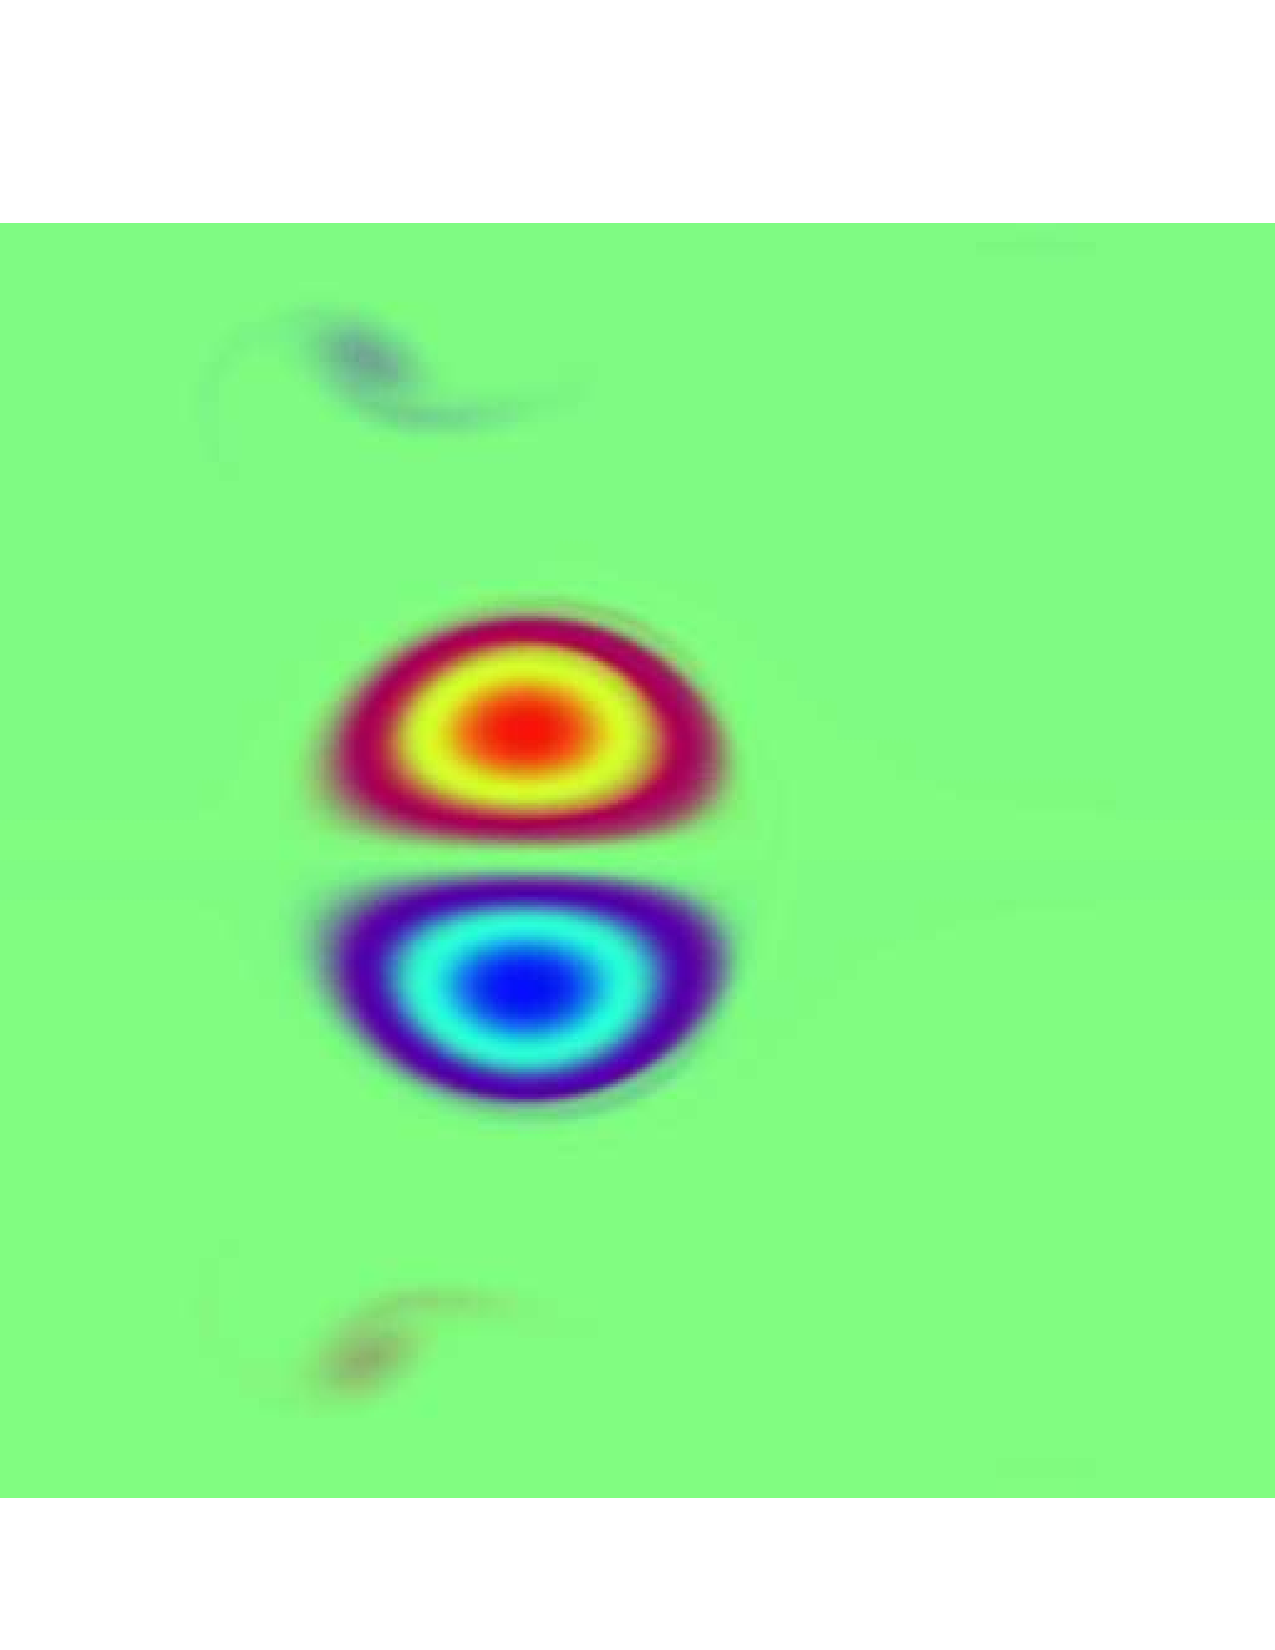
\includegraphics[width=0.4\textwidth]{struc_3}
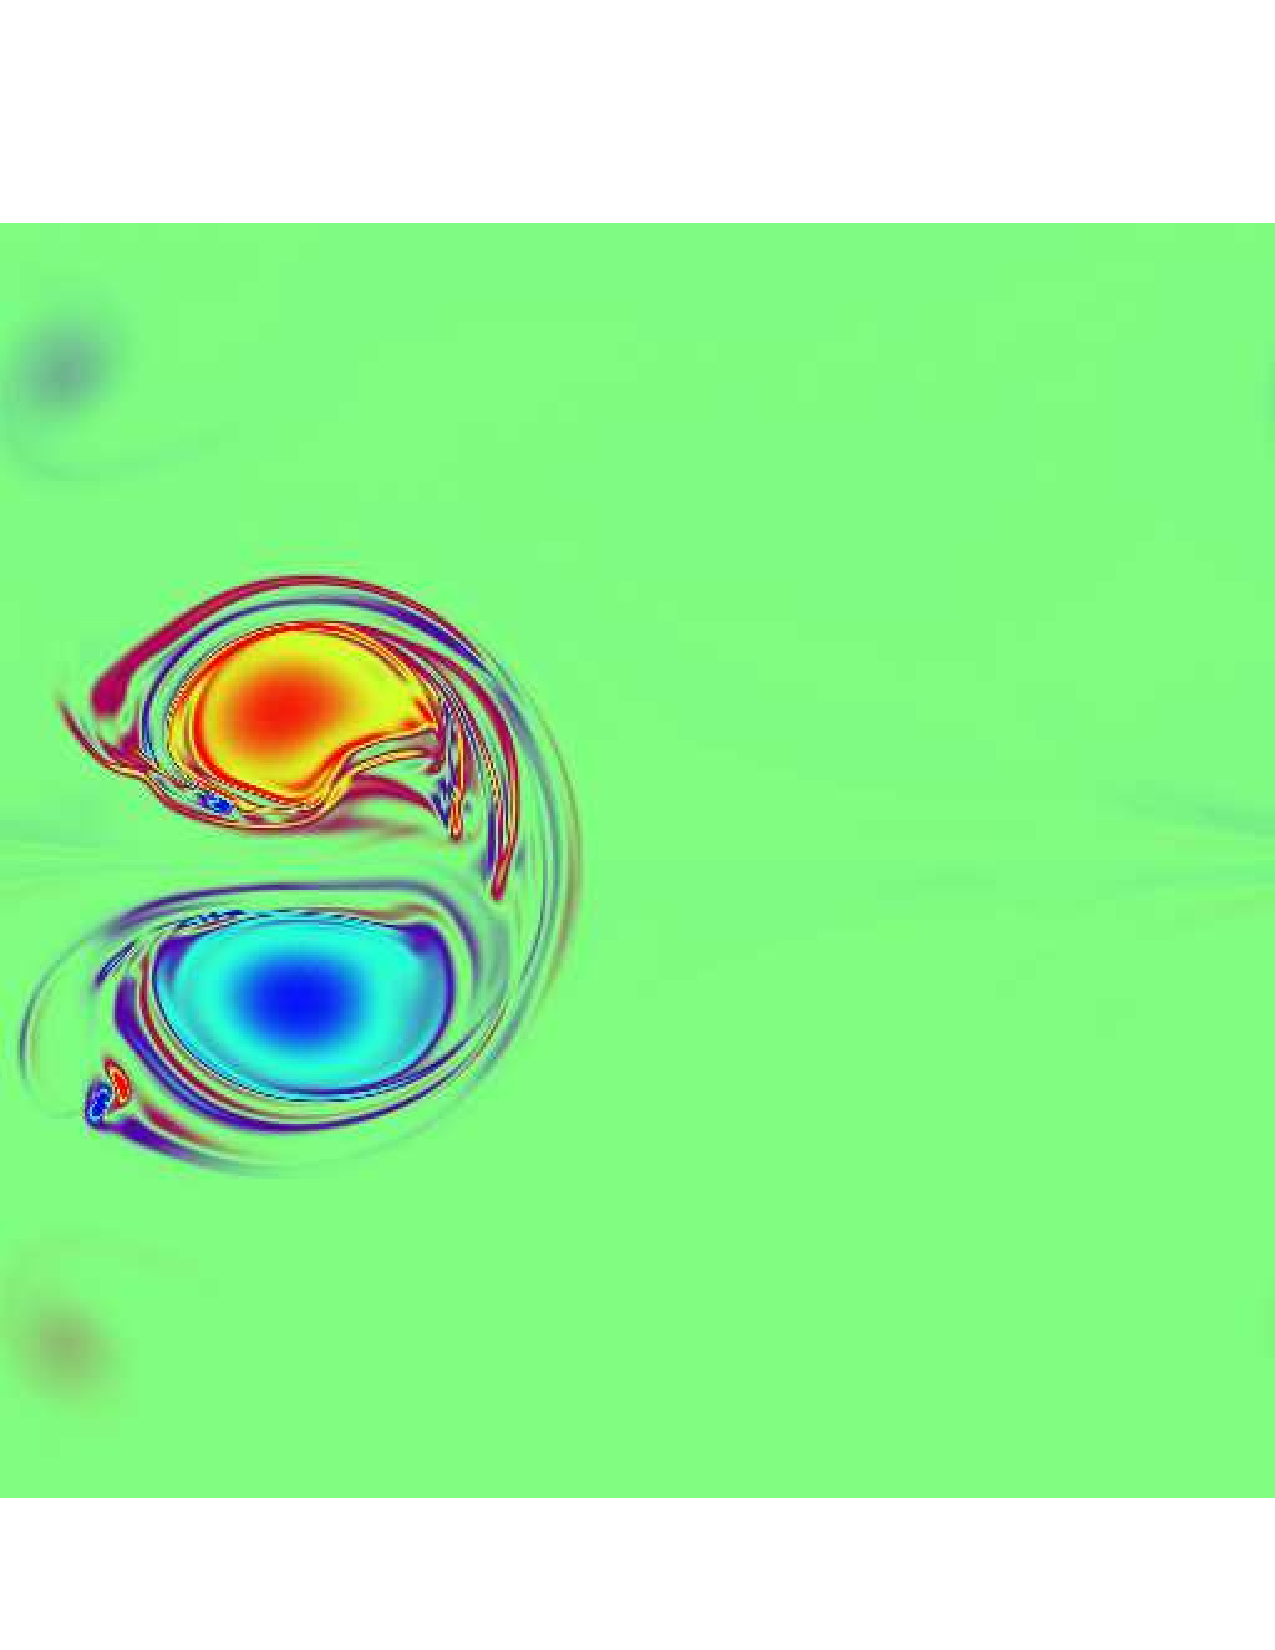
\includegraphics[width=0.4\textwidth]{struc_4}
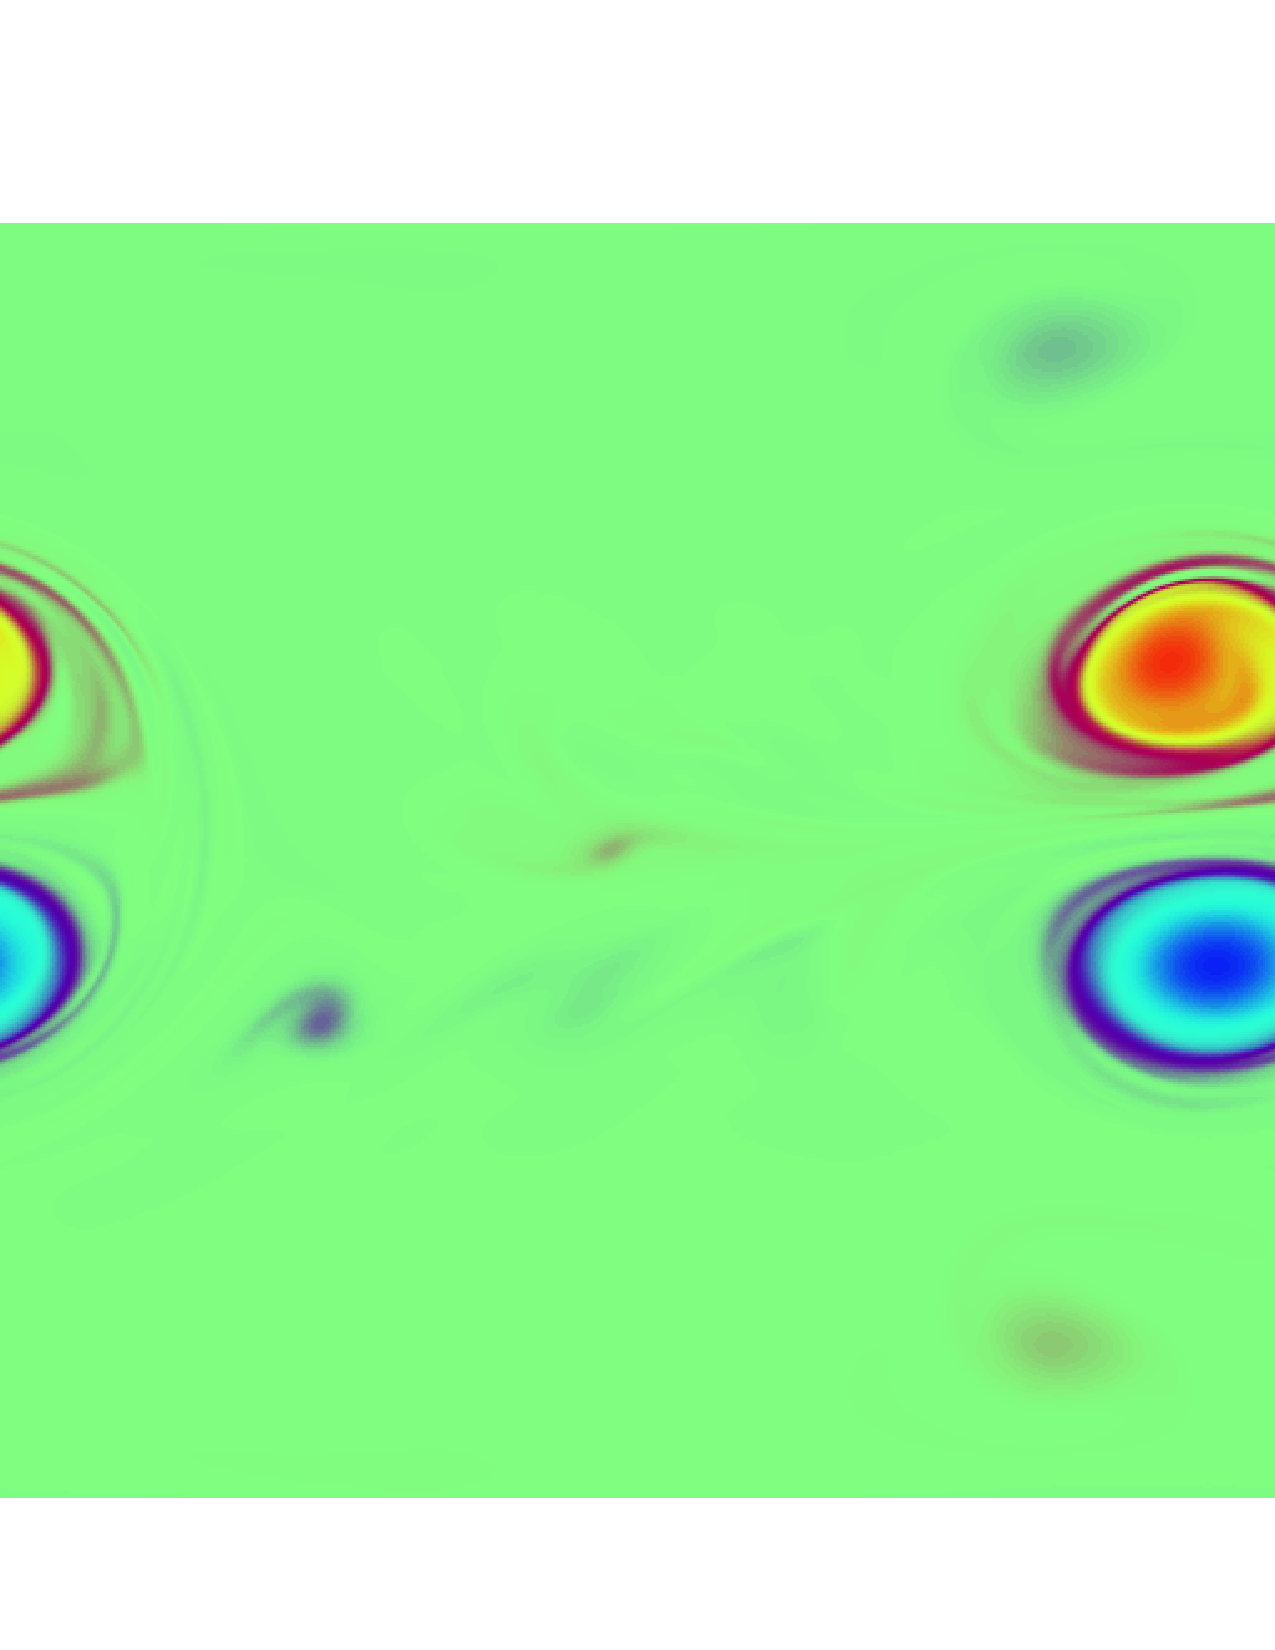
\includegraphics[width=0.4\textwidth]{struc_5}
\caption{Evolution of the vertical vorticity for $Re=5000, F_{h}=0.2, k_{z}=40$ for $T=15$ (top right), $T=20$ (top left), $T=25$ (bottom). Red corresponds to maximum vorticity and blue corresponds to minimum vorticity.}
\label{full_structure}
\end{center}
\end{figure}

We now examine the growth rate of the linear theory compared to that seen in the nonlinear simulations. In comparing the linear theory with the nonlinear theory, there is a problem with what defines the linear regime of the nonlinear simulation. If we examine the growth of the potential energy between $T=5$ and $T=20$ in Fig.~\ref{sat_energy}, it is very difficult to justify approximating this growth rate as linear. For most of the cases of $Re=5000$ and $F_{h}=0.2$, we were unable to determine a consistent way to determine the growth rate of the perturbation and thus we have not included the results for this simulation. For $Re=2000$ and $F_{h}=0.2$, the growth rate of the potential energy was more linear and a linear fit was done to determine the growth rate. Fig.~\ref{growth_rates_nonlinear} illustrates the results for the linear and nonlinear theories for $Re=2000$ and $F_{h}=0.2$. Here the nonlinear growth rates are greater than those of the linear theory; however the shape of the curve follows the linear theory curve reasonably well. Again, the issue of the growth in the potential energy not being perfectly linear could contribute to this discrepancy of $8\%-40\%$. It is unclear why the nonlinear simulations do not exhibit exponential growth, even at early times when the initial perturbation is small. It could be that sub-dominant modes with similar growth rates are contributing to the time series in Fig.~\ref{sat_energy} and the disrepancy with the linear theory, but more work is required to resolve this question. 

\begin{figure}
\begin{center}
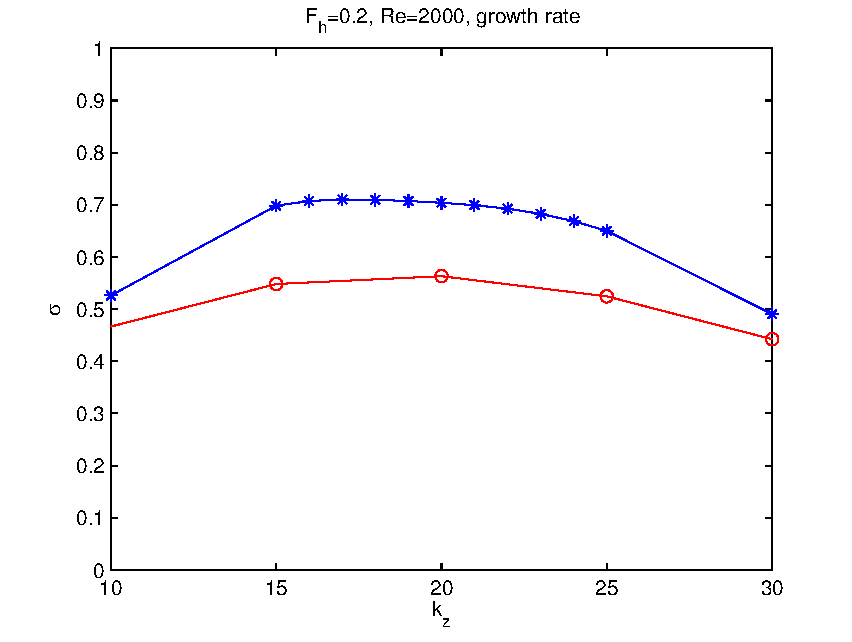
\includegraphics[width=\textwidth]{re2000_fh02_growth_rates} 
\caption{Growth rate for $Re=5000$ and $F_{h}=0.2$ with the linear results (red) and the nonlinear results (blue). Note we have not scaled by $F_{h}$ unlike the results in Chapter 3.}
\label{growth_rates_nonlinear}
\end{center}
\end{figure}

We conclude with a brief discussion of the robustness of the results. To ensure our results were not under-resolved, we ran another simulation with double the horizontal and vertical resolution. In order to keep the computational cost manageable, we shrank the horizontal domain to $L=5$, but kept $n_{x}=1024$, however $n_{z}$ doubled to $64$. The results are plotted in Fig.~\ref{test_energy}. As can be observed, the domain-averaged kinetic and potential energy in the system is higher with $L=5$ because the domain is smaller and hence the dipole takes up a greater percentage of available grid points. Calculating the saturation level, here taken to be the maximum of the potential energy, yields a difference of $2\%$ between $L=5$ and $L=9$. In calculating the growth rate there is a difference of $8\%$. Thus if we increase the resolution, we will obtain similar results. 
\begin{figure}
\begin{center}
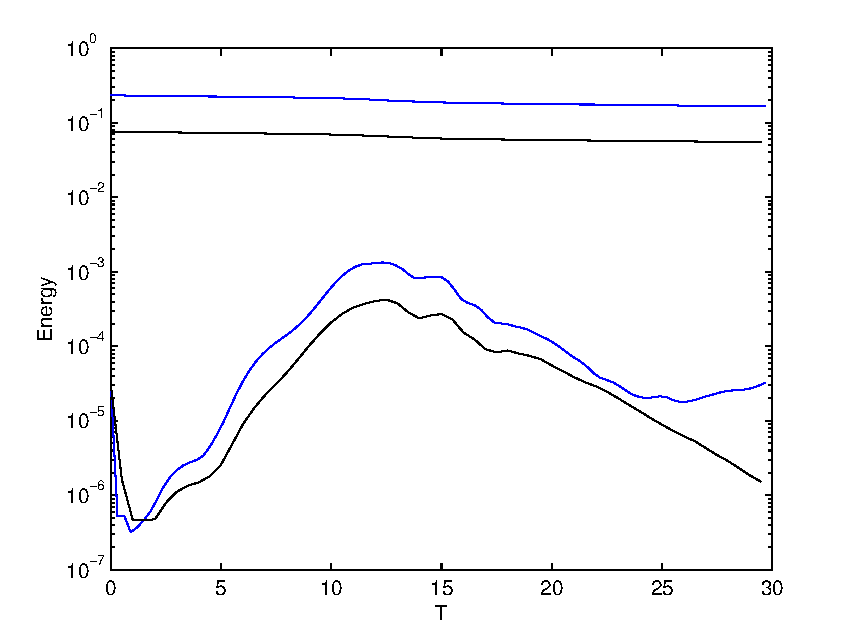
\includegraphics[width=\textwidth]{energy_test}
\caption{Time series of the potential energy (bottom curves) and kinetic energy (top curves) for $L=5$ (blue) and $L=9$ (black). Here $Re=2000, F_{h}=0.2,k_{z}=20$.}
\label{test_energy}
\end{center}
\end{figure}





